Shotwell jest domyślnym menadżerem zdjęć w systemie Ubuntu. Jego zadaniem jest dbanie o organizację twojej kolekcji fotografii i plików graficznych. W chwili pierwszego uruchomienia Shotwell zaproponuje zaimportowanie wszystkich zdjęć z katalogu Obrazy, znajdującego się w twoim katalogu domowym. Fotografie, które później umieścisz w tym katalogu, będa automatycznie dodawane do kolekcji w programie Shotwell.
\begin{center}
	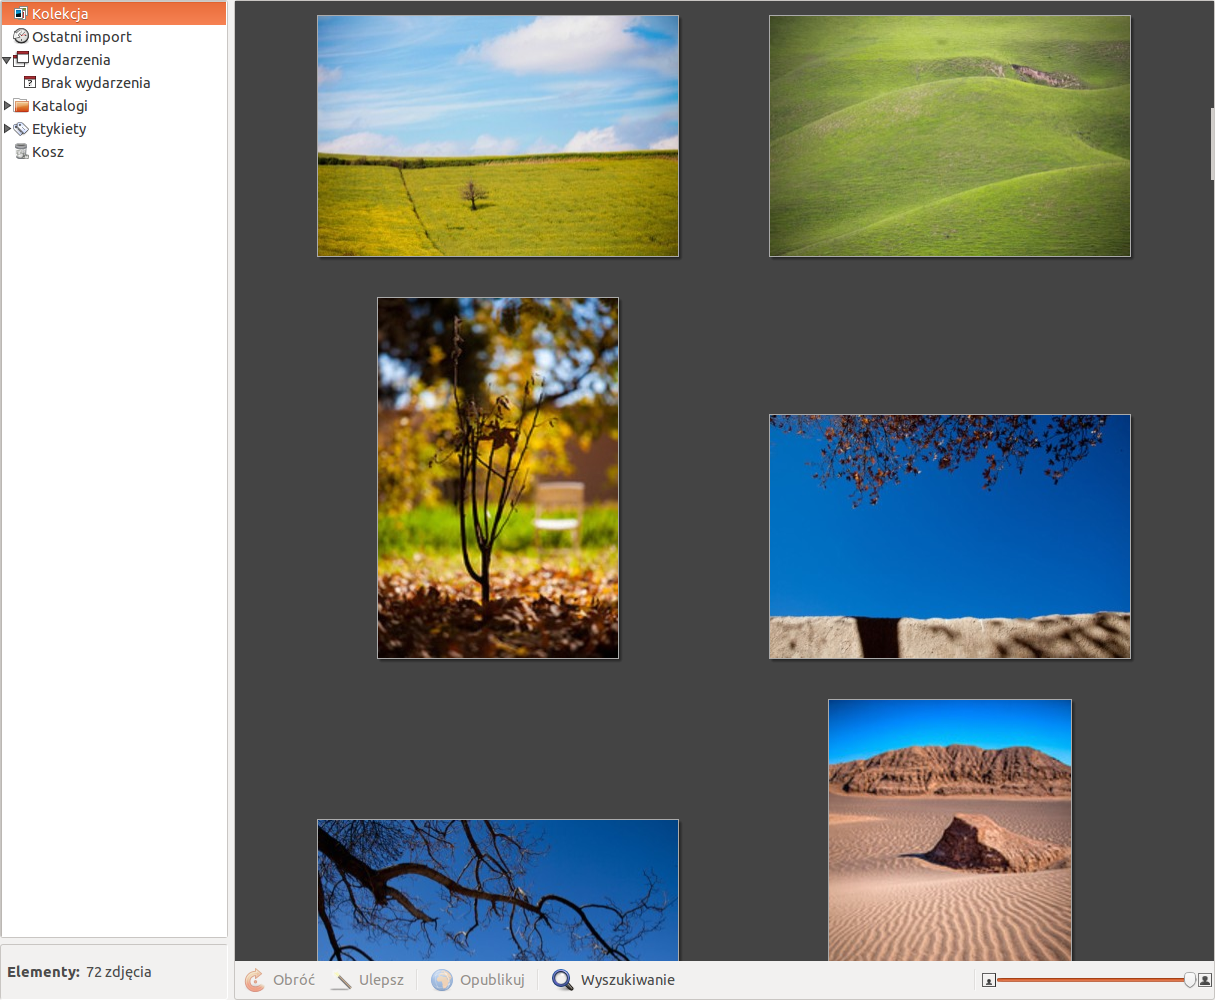
\includegraphics[width=\linewidth]{images/programy_shotwell1.png}
\end{center}

Główne okno programu Shotwell składa się z trzech części:
\begin{itemize}
\item \textcolor{ubuntu_orange}{Lewy panel} zawiera skróty do zaimportowanych katalogów i głównej kolekcji.
\item \textcolor{ubuntu_orange}{Główny obszar} prezentuje obrazy z aktualnie wybranej kolekcji.
\item \textcolor{ubuntu_orange}{Pasek narzędziowy} zawiera narzędzia umożliwiające korekcję zdjęć.
\end{itemize}
\subsubsection{Podstawy obsługi programu Shotwell}
Dodawanie zdjęć do kolekcji
\begin{itemize}
\item Umieść zdjęcia w katalogu Obrazy, by automatycznie dodać je do kolekcji programu Shotwell.
\item Wybierz \menu{{Plik}>{Zaimportuj z katalogu\ldots}}, aby wskazać nowy katalog. Będziesz mieć wybór pomiędzy zwykłym importem ze wskazanego katalogu (zdjęcia zostaną dopisane do twojej kolekcji i pozostaną w oryginalnym katalogu) lub skopiowaniem ich do katalogu Obrazy.
\item Wybierz \menu{{Plik}>{Zaimportuj z programu\ldots}}, aby zaimportować bazę zdjęć z innego programu zainstalowanego w twoim komputerze.
\end{itemize}
Zaznaczanie zdjęć:
\begin{itemize}
\item Kliknij zdjęcie lewym przyciskiem myszy, aby je zaznaczyć.
\item Kliknij dwa razy lewym przyciskiem myszy, aby przejść do widoku pojedynczego zdjęcia.
\item Wciśnij \keys{Shift} i kliknij lewym przyciskiem myszy, aby zaznaczyć wiele kolejnych zdjęć.
\item Wciśnij \keys{CTRL} i klikaj lewym przyciskiem myszy, aby zaznaczyć konkretne zdjęcia.
\item Kliknij prawym przyciskiem myszy, aby wyświetlić menu kontekstowe zdjęcia.
\end{itemize}
Eksport zdjęć:
\begin{itemize}
\item Zaznacz zdjęcia, które chesz wyeksportować.
\item Wybierz \menu{{Plik}>{Wyeksportuj}}, aby wskazać katalog, do którego zdjęcia mają być skopiowane.
\item Wybierz \menu{{Plik}>{Opublikuj}}, aby opublikować zdjęcia w serwisie internetowym. Obsługę dodatkowych serwisów możesz dodać w programie \textcolor{ubuntu_orange}{Konta sieciowe}.
\item Wybierz \menu{{Plik}>{Wyślij do\ldots}}, aby móc wyeksportować zdjęcia do następujących lokalizacji:
	\begin{itemize}
	\item \textcolor{ubuntu_orange}{Dyski wymienne i zasoby sieciowe} --- pozwala wybrać miejsce docelowe w sieci lokalnej lub na lokalnie podłączonych urzadzeniach (np. dysk USB);
	\item \textcolor{ubuntu_orange}{Asystent CD/DVD} --- uruchamia program do wypalania płyt Brasero i umożliwia nagranie wybranych zdjęć na płytę;
	\item \textcolor{ubuntu_orange}{Wiadomość} --- umożliwia wysłanie zdjęć poprzez komunikator internetowy (np. Empathy);
	\item \textcolor{ubuntu_orange}{Bluetooth} --- wysyła zdjecia bezprzewodowo do urzadzeń Bluetooth;
	\item \textcolor{ubuntu_orange}{E-mail} --- otwiera program pocztowy i dodaje zdjęcia jako załączniki.
	\end{itemize}	
\end{itemize}
